\paragraph*{Company Provided Data}
As already mentioned earlier, the \textit{data capture} process is split into two parts.\\
The first part consists of a survey that is sent to and filled out by the human resources department of the company, i.e. the \textit{company provided data}.\\
The questions on this survey will be based on already existing indices, such as the ones from Bloomberg or Equileap.\\
They fill out the survey directly on the website which stores the data on the blockchain via IPFS. Because the data is stored directly on the blockchain, it is visible for everyone and cannot be tempered with in any way at a later point in time.\\
The company also sends us the email addresses of all their employees, which we will store on a private and secure database. The email addresses can obviously not be stored on the blockchain for privacy reasons. This is a tradeoff in transparency that was inevitable.\\

\paragraph*{Employee Survey}
\comment{The employees will now all get an email and not just a percentage of them.\\
This is  done due to the new insight through the interview, where it is suggested that we use all employees for the survey, because a lot of them wont sign up anyway which will lead to a percentage of employees anyways.}
The second part of \textit{data capture}, the \textit{employee survey}, is a special point of interest. Because it is important to guarantee anonymity to the employee and at the same time ensure validity and transparency of the data that is provided.\\

The first step in the \textit{employee survey} takes part after we received all the email addresses of the employees. We send them an email in which there is a link to our survey app.\\
In the app, they enter a password for a new Ethereum blockchain account which gets generated automatically. The private key of the account is stored only on the employees device and is secured by the password they entered. The app sends the public address of the blockchain to our server, where it is used to load a small amount of Ether onto it. This is done, so that the employee can later make one transaction on the Ethereum blockchain.\\
Once all the employees (or a big enough percentage) have followed our link and created an account, our server will create a new survey contract on the blockchain.\\

This happens via the following smart contract (contract \texttt{SurveyFactory}), where an array of public addresses and a hash to the location of the addresses in IPFS is required to create a new smart contract of the kind \texttt{Survey}.\\
\begin{lstlisting}
// https://github.com/EriCreator/bEquality/blob/master/Survey.sol
/*	SurveyFactory serves as a hub 
	(deployed on the blockchain upon the launching of bEquality)
	Company can create their own survey by providing a list of permitted user address. */

contract SurveyFactory {
  mapping(uint => address) public SurveyContracts;
  ...
  function createNewSurvey(uint companyID, address[] addressessOfEmployees, string _hashToaddressessOfEmployees) public returns(address newContract)
  {
    require(SurveyContracts[companyID] == 0x0);
    Survey c = new Survey(addressessOfEmployees, _hashToaddressessOfEmployees);
    SurveyContracts[companyID] = c;
    return c;
  }
  ...
 }
\end{lstlisting}
\texttt{SurveyFactory} can be thought of as a container in which all the surveys of the different companies are stored and can be accessed via the unique id of the company.

After the \texttt{Survey} contract is created, the employees are notified that they now can fill out the survey. They log into their account on the app and answer the questions provided by us. This is done via a user-friendly interface.\\
The survey for the employees presents them with gender specific questions and also with questions applicable for both men and women. These questions guarantee further insight into the microclimate of the employees that cannot be obtained by just consulting the company management.\\
When they submit the data, it gets stored on IPFS and the hash is again stored on the blockchain.\\
This is done via the smart contract \texttt{Survey} seen below. It takes a hash to the location of the survey results on IPFS and stores it on the blockchain.\\
\begin{lstlisting}
// https://github.com/EriCreator/bEquality/blob/master/Survey.sol
/*
   Survey is the child contract created by the SurveyFactory where only the permitted user can modify.
*/

contract Survey {
    mapping (address => string) public hashes;
    mapping (address => bool) public isAllowedToSumbitSurvey;
    string hashToaddressessOfEmployees;

    function Survey(address[] addressessOfEmployees, string _hashToaddressessOfEmployees) public {
        hashToaddressessOfEmployees = _hashToaddressessOfEmployees;
        for (uint256 index = 0; index < addressessOfEmployees.length; index++) {
            isAllowedToSumbitSurvey[addressessOfEmployees[index]] = true;
        }
    }

    function submitResults(string myHash) public {
        require(bytes(hashes[msg.sender]).length == 0);
        require(isAllowedToSumbitSurvey[msg.sender]);
        hashes[msg.sender] = myHash;
    }

}
\end{lstlisting}
The contract ensures that only the employees addresses which were submitted on contract creation can submit results. It also ensures that an employee can only submit results once and that he/she can not alter any other results.\\
Because the employee knows his/her own public blockchain address (it is displayed on the app), he/she can easily verify that the data on the blockchain did not get altered by anybody.\\
The employee is also the only person who knows that this public key is associated to him/her. Thus the sensitive data stored publicly on the blockchain still insures the privacy of the employee and the employer cannot prosecute the employee for telling his opinion on the company.\\

Below the full protocol is shown in a schematic way, to give the reader an overeview of our E-voting protocol.
\begin{figure}[H]
	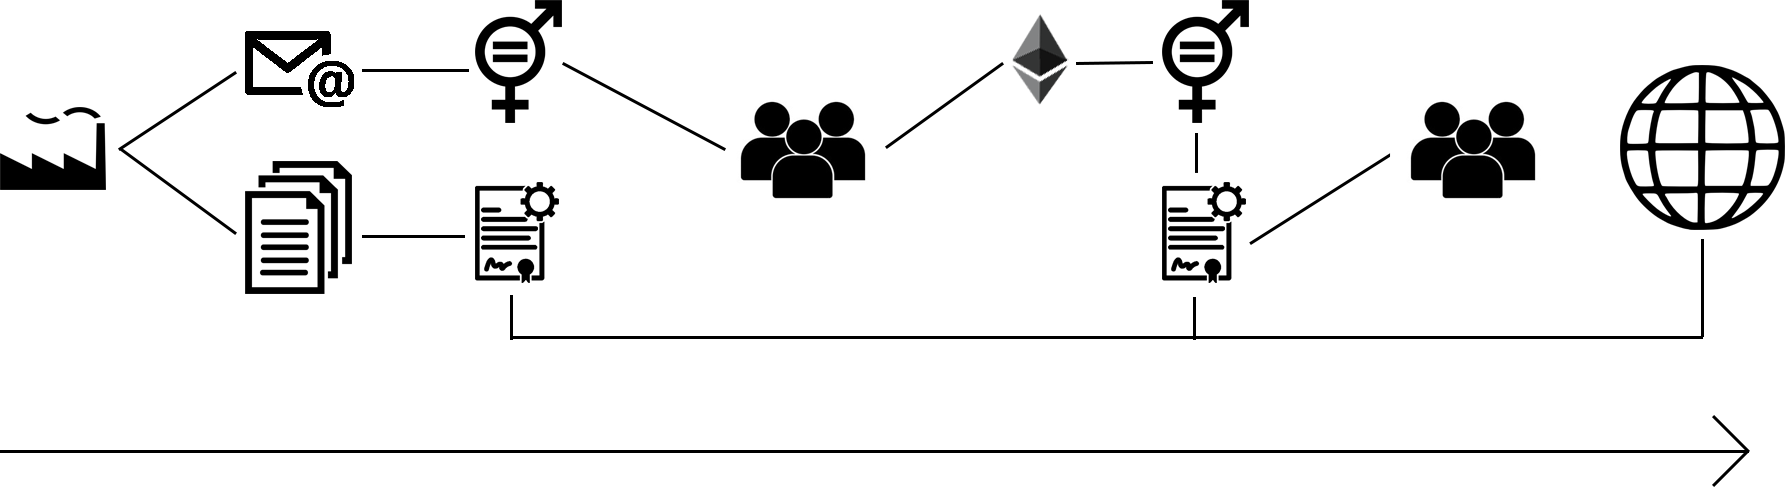
\includegraphics[width=0.9\textwidth]{Bilder/Survey_Protocol_preview_2}
	\caption{technical flow representation of the data capture and storage process}
	\label{technical_flow_representation}
\end{figure}

In our implementation most of the data that gets collected is only stored indirectly on the blockchain via IPFS hashes. This was necessary to reduce the costs of the individual transactions and for overall scalability.\\
Ethereum transaction costs depend, among other things, on the size of the data stored on the blockchain. If we only store hashes instead of survey data, the size of the transaction remains small, no matter the number of questions in the survey.\\

There are still challenges ahead of us for improving our implementation. For example the possibility of storing the public Ethereum addresses on the blockchain instead of a private database while they are still being collected for further transparency and automation of the process.\\

\paragraph*{App Implementation}
To make the survey as easy as possible for the employees, we decided to use an app. We built a demo app for Android smartphones with the Android Studio IDE.\\
The app is only a concept and should serve as a visual guide of how the actual working app would look like. Our demo app consists of a sample survey and dummy buttons and cannot actually submit the survey to the blockchain.\\
Because of the limited time, we were not able to build a working app. Besides the time factor, we did not know how to link the app with the Blockchain/IPFS and if there even is a Java interface to accomplish this task.\\
Nevertheless, our app serves as a great visual reference.\\

\comment{Do not insert pictures as there is a limit of 3 figures in the whole report:
(--insert pictures of the app--)}

The fully implemented app could then work as follows:\\
1. The employee sees a login screen and is asked to fill in his password for the Ethereum blockchain account.\\
2. Once logged in, the app shows the user the questions to answer. The interface is straightforward and self-explanatory.\\
3. After the user submits the survey, the app sends the survey results to the Blockchain/IPFS and reports that the submission was successfull. It also shows the employee his/her blockchain address for verification purposes.\\

The big advantage of an app is the self explanatory user interface.\\

Some of the disadvantages of using an app to collect data are:\\
- Even for one survey, the app needs to be installed on the phones of the employees.\\
- Survey questions are hard-coded into the current app.\\
The second problem can be solved by downloading the questions from a server after the user is logged in. With this approach the app serves as a framework for all kinds of surveys.\\

It is unforeseeable if the app is the right choice to use for the gender equality survey and a good way to find out if it is, would be to test multiple different ways of collecting data and then analysing their effectiveness.\\